
\Lecturer{Hui Jin}
\Contributor{}
\LectureNumber{02}
\LectureDate{DATE}
\LectureTitle{Linear Codes}

\lstset{style=mystyle}

	\MakeScribeTop

%#############################################################
%#############################################################
%#############################################################
%#############################################################
\section{Introduction}
The fundamental problem of channel coding is to encode a stream of message bits into a stream of coded symbols by adding structured redundancy at the transmitter, so that the receiver can use that structure to detect and correct errors. In its simplest form, there is no feedback from the receiver back to the transmitter; this form of channel coding is known as forward error correction.

Forward error correction is the most important technique for fighting the noise present in a communication channel in order to achieve reliable communication. In general, the coded symbols can be binary (taking one of two values) or $q$-ary (taking one of $q$ values, for some integer $q > 2$). In the early days of coding theory, especially in algebraic coding, $q$-ary symbols enabled important coding schemes such as Reed-Solomon codes. However, modern coding methods -- codes defined on sparse graphs, like Low Density Parity Check (LDPC) codes or turbo-like codes -- are usually binary. This does not limit the use of high-order modulation formats in practice: we simply group several coded bits together and map each group onto a modulation symbol before transmission. As a result, $q$-ary symbols have become less central to the theory. In this class we therefore discuss only binary channel coding.

Binary channel coding takes place over the binary field \(GF(2) = \{0, 1\}\): a set of two elements with addition and multiplication defined so that all the usual algebraic rules (associativity, distributivity, etc.) still hold. The only surprising rule is how addition works: \(1 + 1 = 0\). Concretely, this means addition in \(GF(2)\) is the same as the XOR (exclusive-or) operation on bits, and every ``sum'' in this chapter should be read as addition modulo \(2\).

In this chapter, we first discuss various  noisy channel models and two simple coding schemes, the repetition code and the \((7,4)\) Hamming code. Using these two examples, we show the basic concepts such as encoding, decoding. Then we venture into a general framework of block linear codes, the generator matrix for encoding, the parity check matrix for syndrome calculation, and syndrome decoding. 

\section{Noisy Channels}
We limit ourselves to binary input channels. Note that using binary input is a reasonable assumption in low signal-to-noise regimes, (ie noisy channels), as in this scenario, power efficiency is more important. In high signal-to-noise regimes, higher data rate is more important, so spectrum efficiency is more important and we have to use non-binary inputs. 


Therefore we assume the channel has input \(\{0, 1\}\), and output alphabet \(\Sigma_Y\), where \(\Sigma_Y\) can be discrete or continuous. The channel is modeled by the transition probability function \(p(y|x)\), the probability of receiving symbol \(r\) given that the binary value \(x\) is transmitted. 

\begin{example}
    Binary Symmetric Channel (BSC): the output alphabet \(\Sigma_Y\) is \(\{0, 1\}\) and the transition probabilities are:
\begin{align*}
    p(y=0|x=0) &= p(y=1|x=1) = 1- p \\
    p(y=1|x=0) &= p(y=0|x=1) = p
\end{align*}
\begin{figure}[h]
    \centering
    \includegraphics[width=0.5\textwidth]{Figs/BSC_channel.png}
    \caption{Binary Symmetric Channel. Each transmitted bit is flipped with probability \(p\) and received correctly with probability \(1-p\), independently of the other bits. BSC is a good model for channels dominated by random thermal noise.}
    \label{fig:bsc_channel}
\end{figure}

\end{example}

\begin{example}
    Binary Erasure Channel (BEC): the output alphabet \(\Sigma_Y\)  is \(\{0, \star, 1\}\), where \(\star\) represents an erasure. The transition probability are:
\begin{align*}
p(y=0|0) &= p(1|1) = 1 -p \\
p(\star|0) &= p(\star|1) = p
\end{align*}

\begin{figure}[h]
    \centering
    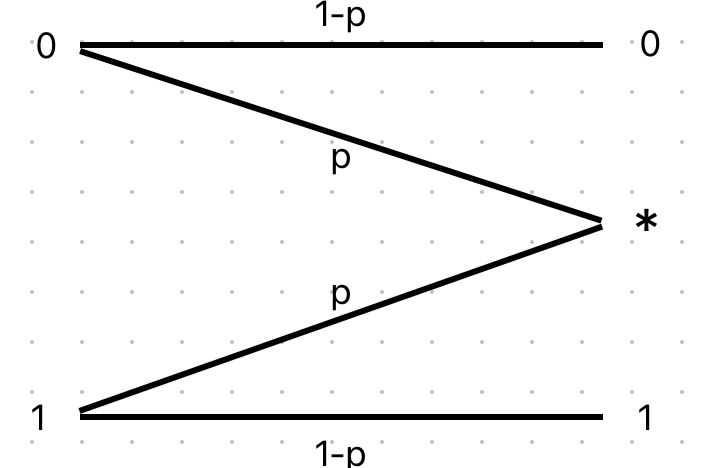
\includegraphics[width=0.5\textwidth]{Figs/BEC_channel.png}
    \caption{Binary Erasure channel. A bit has probability \(p\) erased; otherwise, it is received correctly. BEC is a good model for internet traffic.}
    \label{fig:bec_channel}
\end{figure}

\end{example}

\begin{example}
    Additive White Gaussian Noise Channel (AWGN): here we map bit \(0\) to the transmitted symbol \(+1\) and bit \(1\) to \(-1\) (any fixed mapping between bits and symbols will do). The output value is a Gaussian random variable centered around the transmitted symbol with standard deviation \(\sigma\):
 \begin{align*}
p(y|0) &= \frac{1}{ \sqrt{2\pi\sigma^2}}\; \exp(-(y-1)^2/2\sigma^2) \\
p(y|1) &= \frac{1}{ \sqrt{2\pi\sigma^2}}\; \exp(-(y+1)^2/2\sigma^2) \\
\end{align*}   
Figure~\ref{fig:awgn_channel} depicts the probability distribution given \(\sigma=1\). 

\begin{figure}[h]
    \centering
    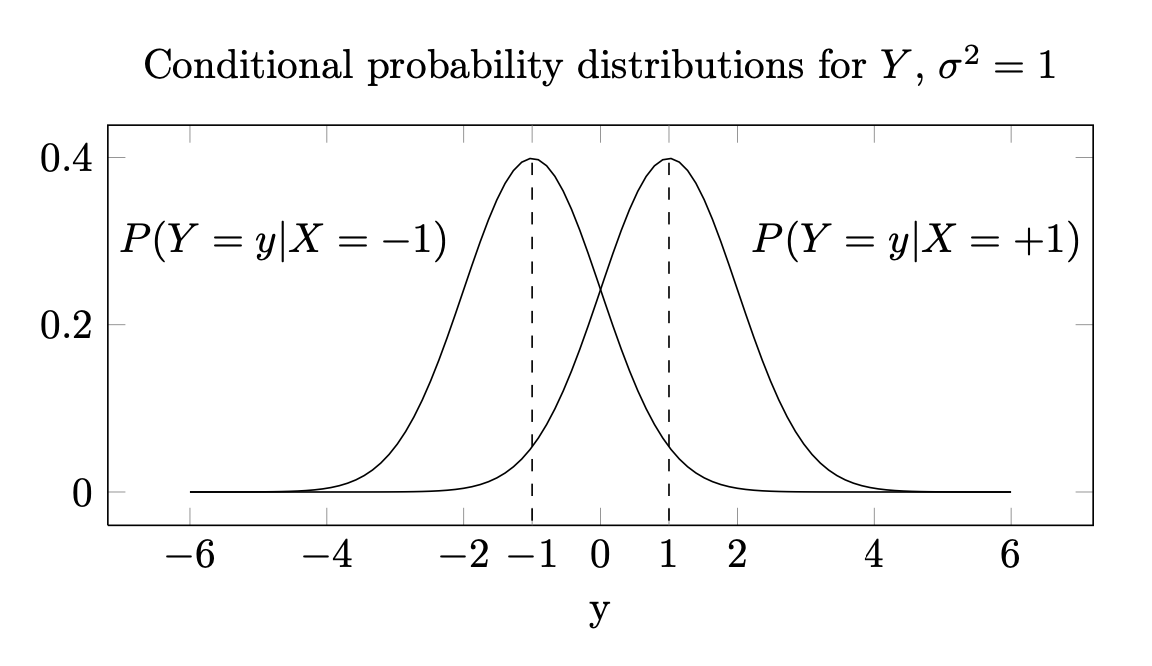
\includegraphics[width=0.5\textwidth]{Figs/BAWGN_pdf.png}
    \caption{Binary Additive White Gaussian Noise channel.}
    \label{fig:awgn_channel}
\end{figure}

The AWGN channel has a continuous output, but a receiver can always fall back to a simple strategy: guess whichever symbol, \(+1\) or \(-1\), is closer to the received value \(y\). This is called making a \emph{hard decision}, and it effectively converts the AWGN channel into a BSC, so it is worth computing the resulting crossover probability \(p\).

By symmetry we may assume the transmitted symbol is \(-1\) and ask for the probability that \(y\) lands closer to \(+1\) than to \(-1\), i.e., that \(y > 0\):
\begin{align*}
    P(-1 \rightarrow +1) &= \frac{1}{ \sqrt{2\pi\sigma^2}}\; \int_{0}^{\infty} \exp(-(y+1)^2/2\sigma^2)\, dy \\
          &= \frac{1}{ \sqrt{2\pi\sigma^2}}\; \int_{1}^{\infty} \exp(-y^2/2\sigma^2)\, dy \\
          &= Q\left(\frac{1}{\sigma}\right)
\end{align*}
where \(Q(\cdot)\) is the standard Gaussian tail probability, i.e., \(Q(x) = P(Z > x)\) for a standard normal random variable \(Z\). This crossover probability \(p = Q(1/\sigma)\) is exactly the BSC parameter that results from hard-decision decoding of the AWGN channel.
\end{example}



\section{Repetition Codes} The simplest coding scheme is a repetition code. 
At the transmitter side, in order to combat noise, we repeat every message bit \(q\) times. Take the example \(q=3\): each message bit is repeated three times. That means we transmit \(000\) if the message bit is \(0\), and transmit \(111\) if the message bit is \(1\). The bits \(000\) and \(111\) are called the code bits. This process of turning \(1\) message bit into \(3\) coded bits is called the encoding process. For a stream of message bits \(10010\), the encoded bit stream will be \(111000000111000\), as illustrated in Figure~\ref{fig:Repeat3}.

\begin{figure}[h]
    \centering    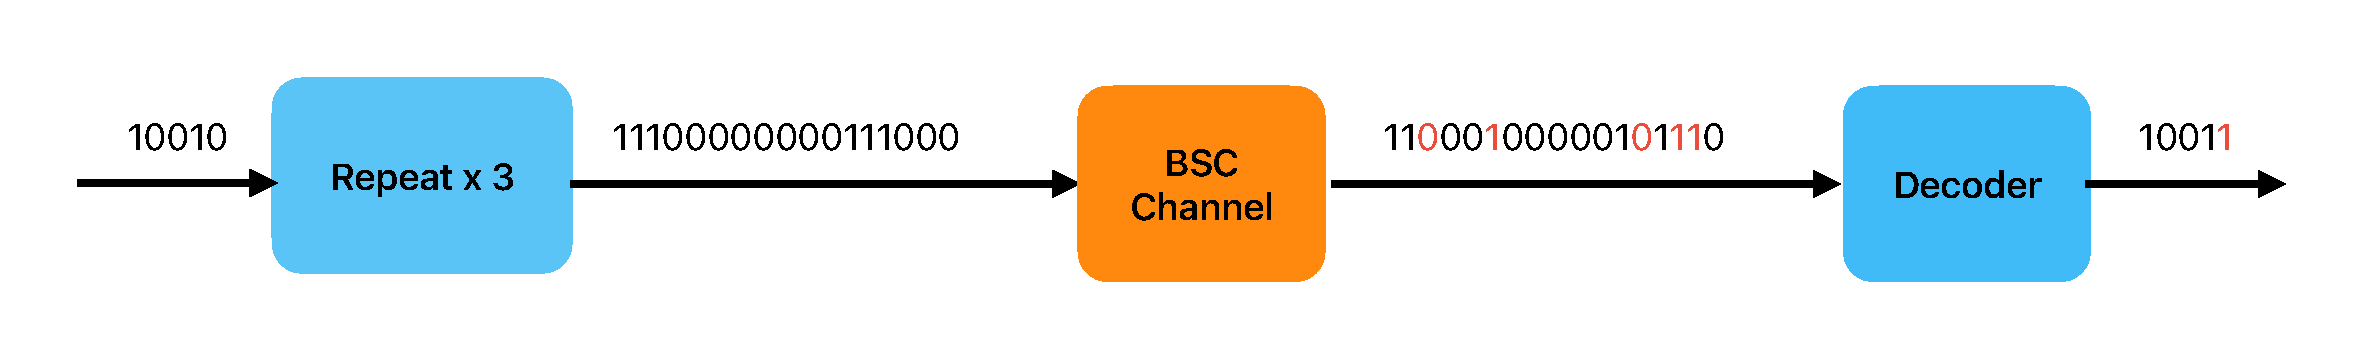
\includegraphics[width=1\textwidth]{Figs/Repeatx3Code.pdf}
    \caption{Encoder and decoder of a Repetition-3 code. The Binary Symmetric Channel (as introduced in the first lecture) has crossover probability \(p\).The decoder is a majority vote decoder for each three coded bits. The decoded message bit has the last bit wrong.}
    \label{fig:Repeat3}
\end{figure}


Let us assume the bits go through a binary symmetric channel with cross-over probability \(p\). Then the receiver, because of the cross-over noise, receives a garbled version, for example, \(110001000101110\), where \(5\) bits are received incorrectly, as indicated by the red color on the bit in Figure~\ref{fig:Repeat3}. The receiver knows that every group of three bits should be identical if there is no noise and it will use that information to decide the correct message bit. This process of using the structured information to infer the right message bit is called the decoding process. 


We first realize the decoding method should decode each message bit separately as there's no information encoded across these bits. So we try to decode the correct message bit given every three coded bits. Assuming the cross-over probability is small, the best decoding method should use a majority vote - the message bit is the bit with the more occurrence. For example, if the received coded bit stream is \(100\), then the message bit is \(0\).

 The message bit will be decoded in error if and only if either two or three of its three copies are flipped by the channel. In the example, the decoded message bit is \(10011\), which we get the last bit wrong. In general, if we use \(P_b^{E}\) denotes the \textbf{bit error probability,} then for repetition code we have:
\begin{align}
    P_b^{E} &= P\{2 \;\text{flips}\} + P\{3 \;\text{flips}\} \nonumber\\
        &= 3p^2(1-p) + p^3 \nonumber \\
        &= 3p^2 - 2p^3. \label{eq:repetitionBER} 
 \end{align}
For \(p < \frac{1}{2}\), the coded bit error probability \(P_b^{E}\) is smaller than \(p\). In fact, for smaller \(p\), the improvement in error probability is significant. 

The improvement of \(P_b^{E}\) over the uncoded system is known as the coding gain. Rigorously, coding gain is defined at a certain error rate and on a particular channel. For example, on the AWGN channel, the difference between the required Signal-to-Noise ratio of a coded system and a uncoded system to achieve a fixed error rate is known as the coding gain for the AWGN channel.   


We can increase the number of repetitions \(q\). In the next we show that as \(q\) goes large, the bit error probability goes to zero. That is we can achieve a reliable communication. Using the argument as in Eq.~(\ref{eq:repetitionBER}) is quite involved; instead we apply the weak law of large numbers.

Let us assume among the \(q\) copies of the message bit, the number of bits get flipped is \(k\) at the receiver,  We will decode correct if \(k < q/2\) by majority vote decoding. Since \(k\) is the number of flips, the weak law of large numbers says the sample mean of the fraction of flips converges to the expected value in probability, or 
\begin{align*}
    \lim_{q} Pr\{|\frac{k}{q} - p| > \epsilon\} = 0.
\end{align*}
 This says as \(q\) goes large, the fraction \(\frac{k}{q}\) converges to \(p\) almost surely. We also know that \(p < \frac{1}{2}\), that means  \(k < q/2\) as \(q\) goes large, which means with probability \(1\) we will be able to decode correctly, in other words,  the decoding error probability goes zero. 



\section{Hamming Code}
Repetition code represents the simplest encoding method; as trivial as it is, it is not efficient. For example for \(q=3\),  every message bit is repeated \(3\) times; the effective rate of information transmission is \(\frac{1}{3}\). Put in a different way, for every information bit, we add \(2\) redundant bits. It can correct 1 flip error. 

Richard Hamming in 1950 introduced a code which could also correct 1-bit error but used less number of redundant (or extra) bits. Hamming code is the first non-trivial error correcting code. Interestingly, Hamming's research happened around the same time as Shannon was inventing the information theory and coding theory. 

The original Hamming code encodes 4 message bits \(x_1, x_2, x_3, x_4\) to 7 coded bits by appending three parity check bits \(x_5, x_6, x_7\):
\begin{align}
 x_5 &= x_2 \oplus x_3 \oplus x_4 \nonumber \\
x_6 &= x_1 \oplus x_2 \oplus x_4 \label{eq:HammingEnc}\\
x_7 &= x_1 \oplus x_3 \oplus x_4 \nonumber 
\end{align}
 
Here \(\oplus\) stands for the XOR operation. We can represent the encoding using a Venn Diagram as depicted in Figure~\ref{fig:HammingVenn}:

\begin{figure}[h]
    \centering    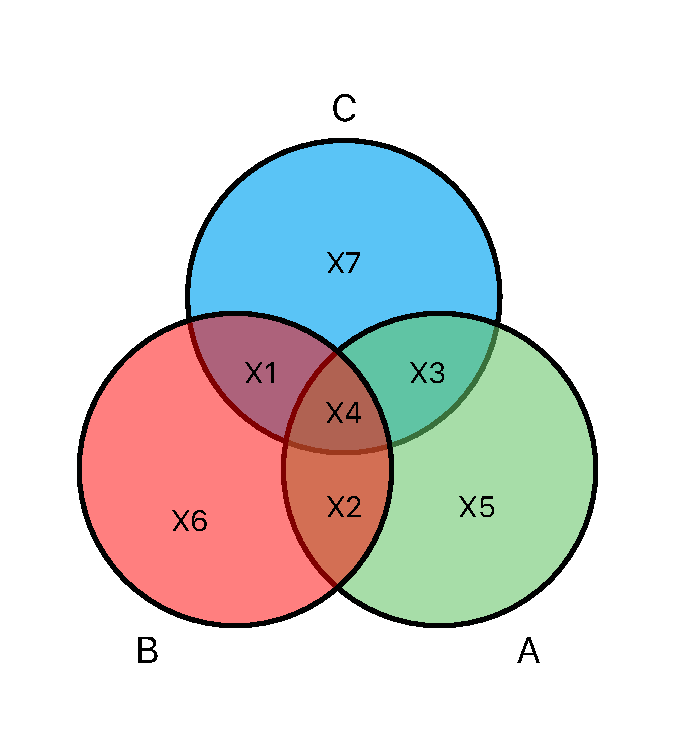
\includegraphics[width=0.6\textwidth]{Figs/HammingVennDiagram.pdf}
    \caption{Venn Diagram of the \((7,4)\) Hamming Code. \(x_1, x_2, x_3, x_4\) are information bits and \(x_5, x_6, x_7\) are parity bits generated. Every circle represents a parity check equation, meaning the sum of the bits in the circle is \(0\).}
    \label{fig:HammingVenn}
\end{figure}




To describe how the receiver recovers the four message bits from the garbled seven-bit codeword, ie the decoding algorithm, we re-write the parity check equations in Eq~\ref{eq:HammingEnc} as 
\begin{align}
   x_2 \oplus x_3 \oplus x_4  \oplus x_5 &= 0 \nonumber \\
 x_1 \oplus x_2 \oplus x_4 \oplus x_6 &= 0 \nonumber \\
 x_1 \oplus x_3 \oplus x_4 \oplus x_7 &= 0  \nonumber
\end{align}
In the Venn diagram Fig~\ref{fig:HammingVenn}, the three parity check equations correspond to circle A, B, and C respectively: all bits in circle A sum up to 0, and so on. 

Now let us form such parity check equations on the received 7-bit vector \(c_1c_2\cdots c_7\) and show that from the result of these three parity checks we are guaranteed to correct one single error:
\begin{align}
   c_2 \oplus c_3 \oplus c_4  \oplus c_5 &= s_1 \label{eq:HamS1} \\
 c_1 \oplus c_2 \oplus c_4 \oplus c_6 &= s_2 \label{eq:HamS2} \\
 c_1 \oplus c_3 \oplus c_4 \oplus c_7 &= s_3  \label{eq:HamS3}
\end{align}

Since there are at most one single error, a satisfying parity check means all bits in the equation is correct; a non-satisfying parity check means exactly one bit in the equation is wrong. From these two facts, we can uniquely determine the flipped bit given the vector \((s_1, s_2, s_3)\).  This fact can be easily seen from the Venn diagram ~\ref{fig:HammingVenn}: if bits in a circle does not sum up to zero, we say that circle is wrong. Then any combination of wrong circles among the three circles uniquely determine a common bit that is included in the wrong circles. If there is at most one single error, this algorithm is guaranteed to succeed. 

\begin{example}
Let us see how we decode the \((7,4)\) Hamming code using a few examples:
\begin{enumerate}
    \item If \((s_1, s_2, s_3) = (1,0,0)\), then the wrong bit only appears in Eq~\ref{eq:HamS1}, or in circle A. That means the bit must be \(c_5\).
    \item If \((s_1, s_2, s_3) = (0,1,1)\), then the wrong bit must participate in both Eqs~(\ref{eq:HamS2},\ref{eq:HamS3}), but not Eq.~\ref{eq:HamS1}. In other words, the bit is only in circle B, and C, but not A. The bit must be \(c_1\).

     \item If \((s_1, s_2, s_3) = (1,1,1)\), then the wrong bit must participate in all these Eqs, that means the bit has to be \(c_4\).
\end{enumerate}
\end{example}


\subsection{Decoding Error Probability of Hamming Code}
Let us consider the error probability that the first message bit \(x_1\) is decoded wrong \(P_{e}^{1}\). (The other bits can be derived similarly). 

Necessarily, but not sufficiently, decoding error happens when there are \(2\) error bits or more among the \(7\) coded bits. We consider the more likely event that there are exactly 2 error bits to get the dominant term. For \(x_1\) to be decoded incorrectly, either \(x_1\) and another bit are flipped, or \(x_1, x_5\) are flipped, or \(x_2, x_3\) are flipped, or \(x_6, x_7\) are flipped. (Refer to the Venn diagram to convince yourself these are the only nine cases for bit \(x_1\) to decode incorrectly.)  There are nine such pairs and this gives the bit error probability 
\begin{align}
    P_{e}^{1} \approx 9 p^2 (1-p)^5. 
\end{align}

Note that this decoding error probability is in the same order as bit error probability of the repetition-\(3\) code Eq.~(\ref{eq:repetitionBER}), at the same time we have \(4\) information bits over every \(7\) coded bits in transmission, a clear advantage. 

\section{Block Codes}
Repetition codes and Hamming codes are two examples of block codes. A block code encode \(k\) information bits to \(n\) coded bits by adding \(n-k\) redundancy bits. There are \(2^k\) codewords among the possible \(2^n\) strings of length-\(n\) binary vector. The essential problem of channel coding is how to effectively select the \(2^k\) codewords such that the we can have good decoding performance while both the encoding and decoding complex is practical.




From our above discussion of repetition codes and \((7,4)\) Hamming code, we know that as it is important for the encoder to make the codewords as far apart as possible as the decoding error depends on the distance between two codewords. A large distance makes it harder for the errors introduced by the channel to cross from a codeword to a nearby distinct codeword. 

For example, for the repetition code with repetition number \(q\), the distance between the two valid codewords is \(q\). So as long as the number of errors is less than \(q/2\), majority vote decoding will recover the correct message bit. So the error probability will decrease as we increase \(q\).

However, a distance property of the codewords imposes a constraint on the number of codewords we can have on the bit-stream of \(n\) bits. Say we want to guarantee a distance property of \(d\), then every codeword excludes all neighboring \(n\)-bit strings within \(d\) distance. That gives an upper bound on the number of codewords. 

We can formalize the question:  Given a minimum distance \(d\) (we shall define it rigorously in the following), what is the maximum number of codewords we can have? This can be understood as picking the maximum number of points on the \(2^n\) lattices so that the distance \(d\) is maintained. In fact, that is exactly the approach we are going to take to derive some heuristic relationship between the number of codewords and the distance property of the codewords.  


Let us first define a few terms which can be used to characterize the properties of codes in general.

\begin{definition}
     The Hamming distance between bit strings \(x\) and \(y\) is defined as the number of positions at which the two strings differ. 

More formally, the Hamming distance \[\Delta(x, y) = |\{i|x_i \neq y_i\}| \]
\end{definition}


\begin{definition}
The Hamming weight of a string \(x\) is defined as the number of non-zero bits in the string.

More formally, the Hamming weight of a string 
\[wt(x) = |\{i|x_i  \neq 0\}|\]
\end{definition} 


\textbf{Remark.} Note that Hamming weight and Hamming distance are directly related: 
\[wt(x-y) = \Delta (x, y).\]


\begin{definition}
A binary error correcting code \(C\) of block length \(n\) is any subset
of \(GF(2)^n\).
    
\end{definition}

\begin{definition}
    A code \(C \subset GF(2)^n\)  is said to have minimum distance \(d(C)\), defined as
\[ d(C) = \min_{c_1 \neq c_2 \in C} \Delta(c1, c2).\]
\end{definition}

Plainly speaking, if \(d(C) = d\), then for every pair of distinct codewords in \(C\), the Hamming distance between them is at least \(d\). And there exists at least two codewords the Hamming distance between them is exactly \(d\).

Given the codeword set \(C\), we can map \(\log_{2}|C|\) message bits uniquely to each of the codeword. Larger number of codewords means more information go through the channel for each codeword. This is the important notion of information code rate:     
\begin{definition}
Information code rate of a binary code \(C\) over with block length \(n\) is defined as 
\[R = \frac{\log_{2}|C|}{n}.\]    
\end{definition}


We sometimes like to normalize the distance of a code to its block length, as we do with rate. To do so, we define the relative distance of a code \(C\), denoted \(\delta(C)\), as the ratio of its distance to its block length:

\[\delta(C) = \frac{d(C)}{n}. \]

\begin{example}
\textbf{Repetition Code}. For a length-\(q\) repetition code, the code rate is \(1/q\) and the minimum distance is \(q\). 
\end{example}

\begin{example}
\textbf{Single Parity Check Code}. The SPC code is generated by adding a redundant parity bit of the other \(n-1\) bits to make a length \(n\) codeword. The code rate is \((n-1)/n\). The parity check code is an example of distance \(2\) code. We can verify that by noticing that all codewords having even weights and there is the all-zero codeword and a codeword with weight \(2\).
\end{example}

\begin{example}
The \((7,4)\) Hamming code discussed earlier is an example of distance \(3\) code. The code rate is \(4/7\). We can verify the distance \(3\) by first showing the difference between two codewords is a codeword, and each codeword has at least hamming weight \(3\). 
\end{example}



\paragraph{Detectable Error} We call a binary error event \(e\) detectable if for any codeword \(c\), the corrupted received vector \(c + e\) is not another codeword. If the code \(C\) has \(d(C)=d\), then any binary error event with weight less than \(d\) is detectable.  

\paragraph{Correctable Error}
We call a binary error event \(e\) correctable if for any codeword \(c\), the corrupted received vector \(c + e\) is closer to another codeword \(c\) than another other codeword. If the code \(C\) has \(d(C)=d\), then any binary error event with weight less than \(\lfloor d/2\rfloor\) is correctable.

We can formalize the above discussion into the following theorem. 
\begin{theorem}
 Consider a binary code \(C\). Then, the following statements are equivalent:
\begin{enumerate}
    \item \(C\) has minimum distance \(2t + 1\);
    \item \(C\) can be used to correct all \(t\) bit errors, but not some \(t+1\) bit errors; 
    \item \(C\) can be used to detect all \(2t\) bit errors, but not some \(2t+1\) bit errors;
    \item \(C\) can be used to correct all \(2t\) erasures, but not some \(2t+1\) erasures.   
\end{enumerate}   
\end{theorem}


\begin{proof}
The proof can be best understood using a geometric visualization. 

Assume statement 1. We can imagine drawing disjoint spheres of radius \(t\) centered at each codeword in \(C\). Such balls are called Hamming balls. Thus, we can uniquely identify the initial codeword from an erroneous string \(s1\) in \(GF(2)^n\) as long as the number of errors is \(\leq t\) by identifying the Hamming ball which contains \(s1\). Additionally, if one or more, but not more than \(2t\) errors occur, then the codeword gets distorted to an erroneous string \(s2\) which must be different from every codeword. Thus such error patterns can be detected. We can also identify up to \(2t\) missing symbols given their positions for any erroneous string \(s3\) by identifying the unique codeword that is consistent with \(s3\).


Assume that statement 1 is false. Thus there exists two codewords \(c_1\) and \(c2\) whose Hamming distance \(d \leq  2t\). 

Consider the midpoint of \(c_1\) and \(c_2\); call it \(x\). The Hamming distance of \(x\) from both \(c_1\) and \(c_2\) is \(\leq t\). 

If \(t\) bit errors are allowed then either \(c_1\) or \(c_2\) could give rise to x. Thus, on the string \(x\) it wouldn’t be possible to correct the errors. Hence \(C\) cannot correct all t symbol errors If \(2t\) symbol errors are allowed then \(c_1\) could give rise to \(c_2\) and thus we cannot be sure that a codeword corresponds to no errors. Hence C cannot detect all \(2t\) symbol errors. If \(2t\) symbols are erased then either \(c_1\) or \(c_2\) could give rise to the same string (take \(c_1\) and erase all positions which are different from \(c_2\)) and thus we cannot correct \(2t\) symbol erasures. 
\end{proof}

\section{Bounds on the size of the Codes}
Obviously, given a fixed \(n\), the higher code rate \(R\) is, the more difficult to have a larger \(d\), or better error protection capability. This is the most fundamental trade-off in codes design.  The following several bounds give a quantitative relationship between code rate and minimum distance. 

\subsection{Singleton Bound}
\begin{theorem}
For a code with minimum distance \(\delta n\), the rate of the code is upper bounded by: 
\begin{align*}
    R \leq 1 - \delta. 
\end{align*}
\end{theorem}

\begin{proof}
We prove that for a code \(C\) to have minimum distance \(d\), then the code size \(|C| \leq 2^{n-d+1}\) by proof by contradiction. If \(|C| > 2^{n-d+1}\), consider the first \(n-d+1\) bits of these codewords, and call it the prefix of a codeword. As there are only \(2^{n-d+1}\) possible prefixes, there are at least two codewords who have identical prefix. But then the distance of these two codewords is at most \(d-1\). Contradiction. 

So \begin{align*}
    |C| &\leq 2^{n-d+1} 
\end{align*}

In the limit \(n\) goes large, we have
\begin{equation}
    R \leq 1- \delta. \label{eq:singletonBound}
\end{equation}
Which says, if minimum distance is a linear fraction of the code block length, then code rate R is upper bounded by \(1-\delta\).    
\end{proof}


The singleton bound is very loose. We can derive much tighter bounds, both in the lower bound and upper bound. Let us consider a much tighter upper bound, the Hamming bound.

\subsection{Hamming Ball}
First, Let us define a Hamming ball \(S_t(c)\) around a codeword \(c\) as the set of length-\(n\) vectors \(e\) such that \(\Delta(e,c) \leq t\), or 
\begin{align*}
    S_t(c) = \{e: \Delta(e,c) \leq t\}
\end{align*}

Let us further define the volume of Hamming ball \(S_t(c)\) as \(Vol(n, t)\), which is independent of \(c\),
\begin{align*}
Vol(n, t) = \sum_{i=0}^{t}  \binom{n}{i}.    
\end{align*}

\begin{lemma} 
Vol(n, pn) is well approximated by \(2^{H(p) n}\), where \(H(x)\) is the binary entropy function, 
\[H(x) = - x \log_2(x) - (1-x) \log_2(1-x).\]

In other words, 
\(log_2 Vol(n, pn) \approx H(p) n.\)
\end{lemma}

\begin{proof}
We have 

\begin{align*}
Vol(n, pn) &= \sum_{i=0}^{np}  \binom{n}{i} \\           & \sim   \binom{n}{np}\\
        &\sim \frac{\sqrt{2\pi n} (n/e)^n} {\sqrt{2\pi np} (np/e)^{np} \sqrt{2\pi n(1-p)} (n(1-p)/e)^{n(1-p)}}  \\
        &\sim \frac{1}{p^{np}(1-p)^{n(1-p)}}  \\
        &= 2^{H(p) n}
\end{align*}
\end{proof}
where in the second approximation we use the Stirling formula: 
\[
m! \sim \sqrt{2\pi m} (m/e)^{m}.
\]

\subsection{Hamming Bound}
 The following Hamming bound improves the singleton bound considerably. In fact, in some cases, it is achievable.

\begin{theorem}
For a code with minimum distance \(\delta n\), the rate of the code is upper bounded by: 
\begin{align*}
    R &\leq 1 - H(\delta). 
\end{align*}
\end{theorem}
We know \(S_t(c_1)\) and \(S_t(c_2)\) cannot be overlapping for every pair of codewords \(c_1, c_2\) if the code is able to correct upto \(t\) errors.   

However, there are only \(2^n\) possible vectors in the whole Hamming space, therefore the number of codewords is upper bounded by:
\begin{align*}
    |C| \cdot Vol(n, t) &\leq 2^n \\
    \log_2 |C| + \log_2 Vol(n, t) &\leq n \\
    R &\leq 1 - H(t/n) 
\end{align*}
This is also called the sphere packing bound due to the argument above. Note that in the limit, \(t/n = \frac{d}{2n} = \delta/2\), we have
\begin{align*}
    R &\leq 1 - H(\delta/2). 
\end{align*}

The Hamming bound makes precise the intuitively obvious fact that error correcting codes can not achieve arbitrarily high rate \(k/n\) while still retaining a linear minimum distance. 

\subsection{Gilbert-Varshmov Bound}
It can be shown that for given \(n, d,\) there exists a linear \([n, k, d]\) code provided
\begin{align*}
2^k \sum_{i=0}^{d-1}\binom{n}{i} < 2^n    
\end{align*}
In the limit of large \(n, k, d,\) and putting \(t = d/2,\) this becomes
\begin{align}
    \frac{k}{n} \geq (1 - H(\frac{2t}{n}))(1-\eta)    \label{eq:GVBound}
\end{align}
where \(\eta \rightarrow 0\)  as \(n \rightarrow \inf\). It can be shown that there exists an infinite sequence of \([n, k, d]\) codes satisfying 
\ref{eq:GVBound} with \(d/n \geq \delta\) if \(\delta < 1/2\). The Gilbert-Varshamov bound necessarily lies below the Hamming bound, but it is an important result because it shows that error correction can be very powerful.

Note that in the limit, \(2t/n = \frac{d}{n} = \delta\), we have
\begin{align*}
    R &\geq 1 - H(\delta). 
\end{align*}

We can plot the singleton, Hamming, and Gilbert-Varshmov bound together. 

\section{Linear Codes}
If we focus on linear codes instead of general block codes, we impose more symmetry and the code structure can be described more succinctly. Surprisingly, the linear constraint does not compromise code performance at all. 

\begin{definition}
If \(C \subset GF(2)^n\) is a subspace of \(GF(2)^n\) then \(C\) is said to be a linear code.
\end{definition}

The linear property makes all codewords symmetric in the sense that from the point of view of any codeword, the relative position of other codewords is identical to that from the all zero codeword.  This is because from any codeword \(c\), the difference between \(c\) and another codeword \(c'\) is exactly identical to the difference between \(c-c'\), which is a codeword, and the all zero codeword. That means the decoding error probability is independent of the codeword, and therefore in decoding analysis or simulation we can assume the all zero codeword is transmitted.


As \(C\) is a subspace, from basic linear algebra theory, there exists a basis \(c_1, c_2, \ldots, c_k\) where \(k\) is the dimension of the subspace. Any codeword \(c\) can be expressed as the linear combination of these basis vectors, ie 
\[c = \sum \alpha_i c_i, \]
where \(\alpha_i \in \{0,1\}.\) 


\subsection{Generator Matrix}
One way to describe the linear code of dimension \(k\) is through the matrix consisting of the \(k\) basis vectors \(c_1, c_2, \cdots, c_k\) as the columns. We call it the generator matrix \(G\). 



\paragraph{Generator matrix} Given an \(n \times k\) generator matrix of full rank \(G\), we define a linear code:
\[ \{Gx \;|\; x \in GF(2)^k \}.\]
 Here we use the convention that codeword is generated by \(Gx\), where \(x\) is a column vector; some books prefer to use \(xG\), where \(x\) is a row vector. Clearly in that case, \(G\) then is a transpose of the \(G\) defined here.


A linear code with block length \(n\), dimension \(k\) and minimum distance \(d\) will be denoted compactly as an \([n, k, d]\) code, where we may omit \(d\) if its value is understood, unknown, or not relevant to the discussion.

The code rate for a \([n, k, d]\) code is simply \(R= k/n\).

\begin{example}
Generator matrix for the repetition\(-3\) code: 
$$G = \begin{bmatrix}
    1 \\
    1 \\
    1
\end{bmatrix}$$
Encoding is \(c = Gx\).
\end{example}

\begin{example}
Generator matrix for the \((7,4)\) Hamming code. 

 
$$G = \begin{bmatrix}
    1 & 0 & 0 & 0\\
    0 & 1 & 0 & 0\\
    0 & 0 & 1 & 0\\
    0 & 0 & 0 & 1\\
    0 & 1 & 1 & 1\\
    1 & 1 & 0 & 1\\
    1 & 0 & 1 & 1
\end{bmatrix}$$
Encoding is \(c = Gx\), mapping a length-4 column vector \(x = [x_1 x_2 x_3 x_4]^T\) to a length-7 vector \(c = G x\) (the operations are done over modulo 2) where \(G\) is the matrix.
\end{example}



The repetition-3 code we discussed earlier is a trivial \([3, 1, 1]\) linear code; the Hamming code we discussed earlier is a linear code and can be represented as \([7, 4, 3]\) code.


As we have seen a linear code \([n, k, d]\) forms a subspace and the generator matrix \(G\) is used to define the subspace uniquely. 




\subsection{Parity Check Matrix}
Another way of defining the subspace \(C\) in \(GF(2)^n\) is to use its null space. The nullspace of \(C\) is defined as all vectors which are orthogonal to every vector in \(C\). This is equivalent to all vectors which are orthogonal to every column vector in the generator matrix \(G\).

Consider the linear equation system \(xG=0\), the solution space of \(x\) has dimension \(n-k\) from basic linear algebra. This is the null space. We denote the null-space as the subspace \(C^{\perp}\). We can call a matrix consisting a basis of supporting vector of this subspace as a generator matrix for \(C^{\perp}\).


Let \(H\) represent of such \((n-k)\times n\) generator matrix of \((C^{\perp})\). The matrix \(H\) is called the parity check matrix and can also be used to uniquely define the code \(C\). In particular, we can define the code \(C\) as all vectors \(c\) satisfying the following condition: 
\[H c = 0.\]

\begin{example}
Parity check matrix for the repetition\(-3\) code: 
$$H = \begin{bmatrix}
    1 & 1 & 0 \\
    1 & 0 & 1 \\
\end{bmatrix}$$
The parity checking means \(Hc = 0\).
\end{example}

\begin{example}
The parity check matrix for the \((7,4)\) Hamming code is:
$$H = \begin{bmatrix}
    0 & 0 & 0 & 1 & 1 & 1 & 1\\
    0 & 1 & 1 & 0 & 0 & 1 & 1\\
    1 & 0 & 1 & 0 & 1 & 0 & 1
\end{bmatrix}$$
We can easily verify each codeword \(c\) in the Hamming code defined by the generator matrix satisfies the equation \(Hc=0\).
\end{example}

One benefit of using the parity check matrix is the minimum distance property of the code is directly linked to the rank of the column vectors of \(H\). This leads to a crude bound on the minimum distance of a linear block code.


\begin{theorem}
The minimum distance of code \(C\) with parity check matrix \(H\) is the smallest number \(d\) such that there exist \(d\) columns of \(H\) which are linearly dependent.
\label{theo:minDistance}
\end{theorem}

\begin{proof}
     The minimum distance of a linear code is equal to the smallest possible weight of a non-zero code. This is true as a linear code must include all zero codeword and the distance property is symmetric across all codewords. Let \(x\) be a non-zero code of smallest weight \(d\). We know that \(Hx = 0\), therefore there exists \(d\) linearly dependent columns of \(H\). Additionally for every set of dependent columns in \(H\) there exists a non-zero code in \(C\) such that \(Hc=0\). Thus, the minimum distance of \(C\) is exactly equal to the size of the smallest linearly dependent column set of \(H\).
\end{proof}

\begin{proposition}
    Let \(C[n,k,d]\) be a code. Then \(d \leq n-k+1\).
\end{proposition}
\begin{proof}
We know the column rank equals to the row rank for any matrix. The rank of the row vectors  of the parity check matrix is at most the number of rows, which is \(n-k\). So any \(n-k+1\) columns are linearly dependent. By theorem~\ref{theo:minDistance}, the minimum distance \(d\) is at most \(n-k+1\).
\end{proof}
    

\subsection{Parity Check Matrix vs Generator Matrix}
The codeword set is the linear combination of the column vectors of the generator matrix \(G\). Without loss of generality, we can permute the rows of \(G\) (which involves changing the ordering of the bits) and with row Gaussian elimination  convert the \(G\) into the following form: 
$$G = \begin{bmatrix}
    I_{k} \\
    P
    \end{bmatrix}
$$
where \(P\) has dimension \(n-k\) by \(k\). 

\begin{theorem}
If the generator matrix \(G\) is in the form: 
$$G = \begin{bmatrix}
    I_{k} \\
    P
    \end{bmatrix}
$$
Then one parity check matrix H is:
\[H = [P \; I_{n-k}]\]
\label{thm:HfromG}
\end{theorem}


\begin{proof}
We check directly that \(H\) annihilates every column of \(G\) (all arithmetic below is over \(GF(2)\)):
\[
HG = [P \; I_{n-k}] \begin{bmatrix} I_k \\ P \end{bmatrix} = P I_k + I_{n-k} P = P + P = 0.
\]
So every codeword \(c = Gx\) satisfies \(Hc = HGx = 0\), meaning \(H\) defines the null space of \(G\); that is, \(H\) is a valid parity check matrix for the code generated by \(G\).
\end{proof}

\section{Dual Code}
We can define a dual code of \(C\), denoted by \(C^{\perp}\) by swapping the role of generator matrix \(G\) and parity check matrix \(H\). That is, we define a code with generator matrix \(G_{dual} = H^T\), where \(H^T\) is the transpose of \(H\). \(H^T\) has dimension \(n \times (n-k)\), therefore the encoding \(x = G_{dual} m\) encodes a \((n-k)\)-bit vector to \(n\)-bit codeword. There are \(2^{n-k}\) codewords. The parity check matrix of the dual code \(H_{dual}\) is \(G^T\). 

Intuitively, this lemma says that if you sum a sign \((-1)^{y\cdot z}\) over every codeword \(y\) in \(C\), the terms either all reinforce each other and add up to the size of the code (when \(z\) belongs to the dual code), or they cancel out perfectly and sum to zero (otherwise). This identity -- relating a linear code and its dual -- will be used later in deriving the decoding capability of CSS codes. 

\begin{lemma}
    Consider a \((n,k)\) linear code \(C\), for a \(n\)-bit vector \(z\), we have  
    \[
     \sum_{y \in C} (-1)^{y \cdot z} =
     \begin{cases}
    |C|, & \text{if } z \in C^{\perp} \\
    0.  & \text{otherwise}
    \end{cases}
    \]
\label{lemma:IdentityDual}
\end{lemma}

\begin{proof}
    If \(z \in C^{\perp}\), then \(y \cdot z = 0\) for any \(y \in C\), so \(S(z) = \sum_{y \in C} (-1)^0 = |C|. \)

    Now consider the non-trial case \(z \notin C^{\perp}\). We know the codespace \(C\) is an abelian group.  The dot product \(\phi_z(y) = y\cdot z\) is a group homomorphism\footnote{The function \(h : G(\star) \rightarrow H(\cdot)\) is a group homomorphism if whenever
\(a \star b = c\)  we have   \(h(a) \cdot h(b) = h(c).\)
In other words, the group H in some sense has a similar algebraic structure as G and the homomorphism h preserves that.
}: \(C \rightarrow Z_2\). This map is surjective when \(z \notin C^{\perp}\), which means that \(K = kernel(\phi_z(y))\) is an index two  subgroup of \(C\). The two cosets - one mapping to \(0\), the other mapping to \(1\) - have the same size. (Another way to see this is that given an element \(s \in C\) where \(\phi_z(s) = 1\), we have for any \(y \in C\) if and only \(\phi_z(y) = 0\) then \(\phi_z(y + s) = 1\), which means the whole set of codewords can be partitioned into two equal size sets whose elements are mapped to \(0\) and \(1\) respectively.) Therefore \(|K|=|C|/2\) and the result follows.

    Alternatively, the non-trial trial case \(z \notin C^{\perp}\) can be explained as the following.

    Assume \(c_0\) is one codeword in \(C\) such that \(c_0 \cdot z = 1\). Then if \(c_1\cdot z = 0\), we have \((c_0 + c_1)\cdot z = 1\);
    if \(c_1\cdot z = 1\), we have \((c_0 + c_1)\cdot z = 0\). That means the whole codewords is partitioned into two groups of equal size such that one group has \(c\cdot z = 0\) and the other group \(c \cdot z =1\) and the result follows.
    This is basically the plain language explanation of the homomorphism proof.
\end{proof}

\subsection{Dual codes of some codes}
\textbf{Dual of the repetition code.} As Exercise 2 below asks you to verify, the dual of the length-\(q\) repetition code is the single parity check code of the same length: its parity check matrix is exactly the \(1\times q\) all-ones generator matrix of the repetition code, and its generator matrix is exactly the repetition code's parity check matrix.

\textbf{Dual of the Hamming code.} The dual of the \((7,4)\) Hamming code is the \([7,3]\) \emph{simplex code}: every nonzero codeword has Hamming weight exactly \(4\), and any two distinct nonzero codewords are at distance \(4\) from each other. (You are encouraged to verify this using the generator and parity check matrices given earlier in this chapter.)

\section{Exercise}
\begin{enumerate}
    \item Prove a code \(C\) with minimum distance \(d\) can correct any \(a\) erasures and \(b\) errors if and only if \(d \geq a + 2b +1\).
    \item Write down the parity check matrix of the dual code for the repetition code? 
    \item The dual code for the repetition code is known as the single parity check code. Determine the number of codewords for a length-n single parity check code. 
    \item Extension from \(GF(2)\) to \(GF(5)\). Assume a codeword is a string of numbers \(x_1x_2\cdots x_n\), where \(x_i \in \{0, 1, 2, 3, 4\}\) and \(x_1 + x_2 + \cdots + x_n = 0 \pmod 5\). Determine the number of such codewords.
    \item Prove theorem \ref{thm:HfromG}.
\end{enumerate}


